Network Statistics:
    88408 nodes
	121946 edges



Figure\ref{fig:chicago}


\begin{figure}[h!]
    \centering
    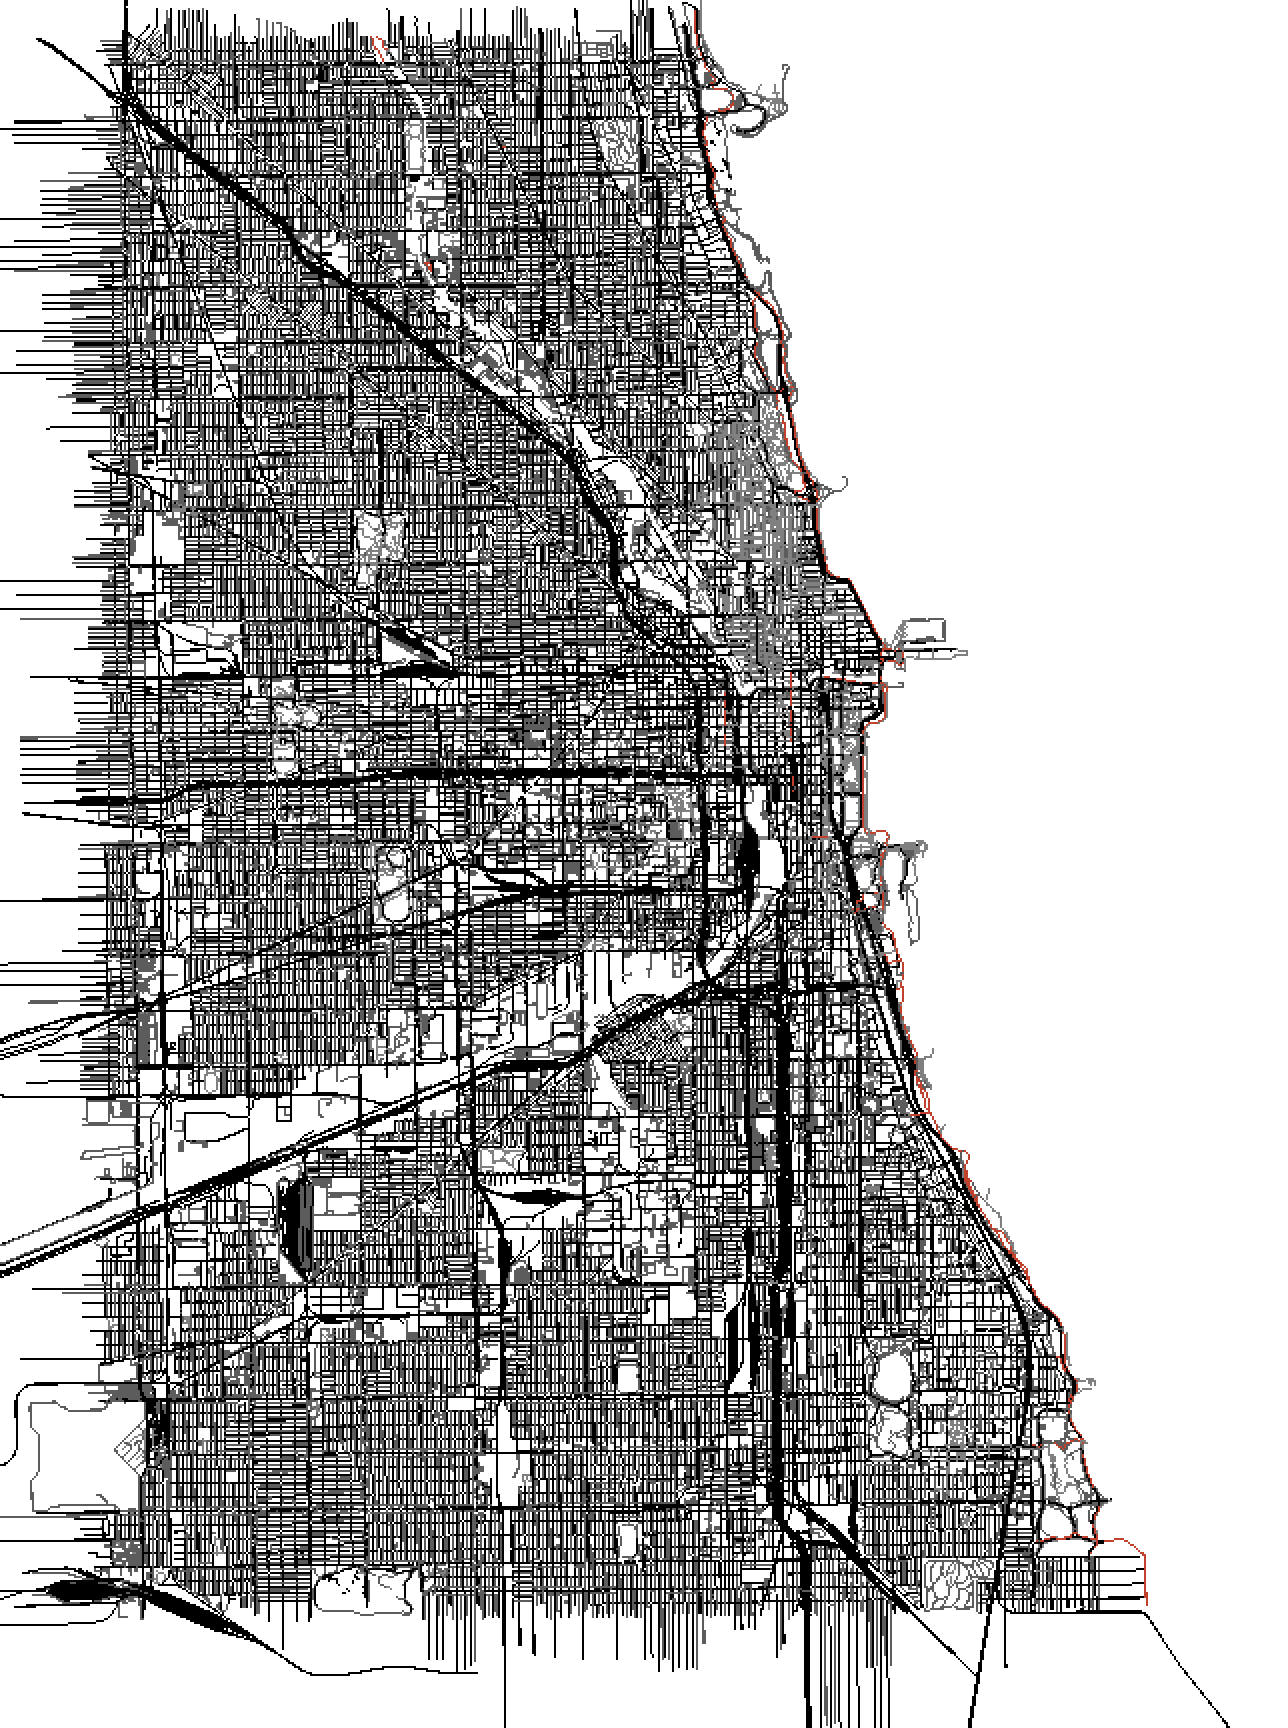
\includegraphics[height=3in]{figs/Chicago_Net_Black_White.png}
    \caption{CAPTION.}
    \label{fig:chicago}
\end{figure}


\begin{figure}[h!]
    \centering
    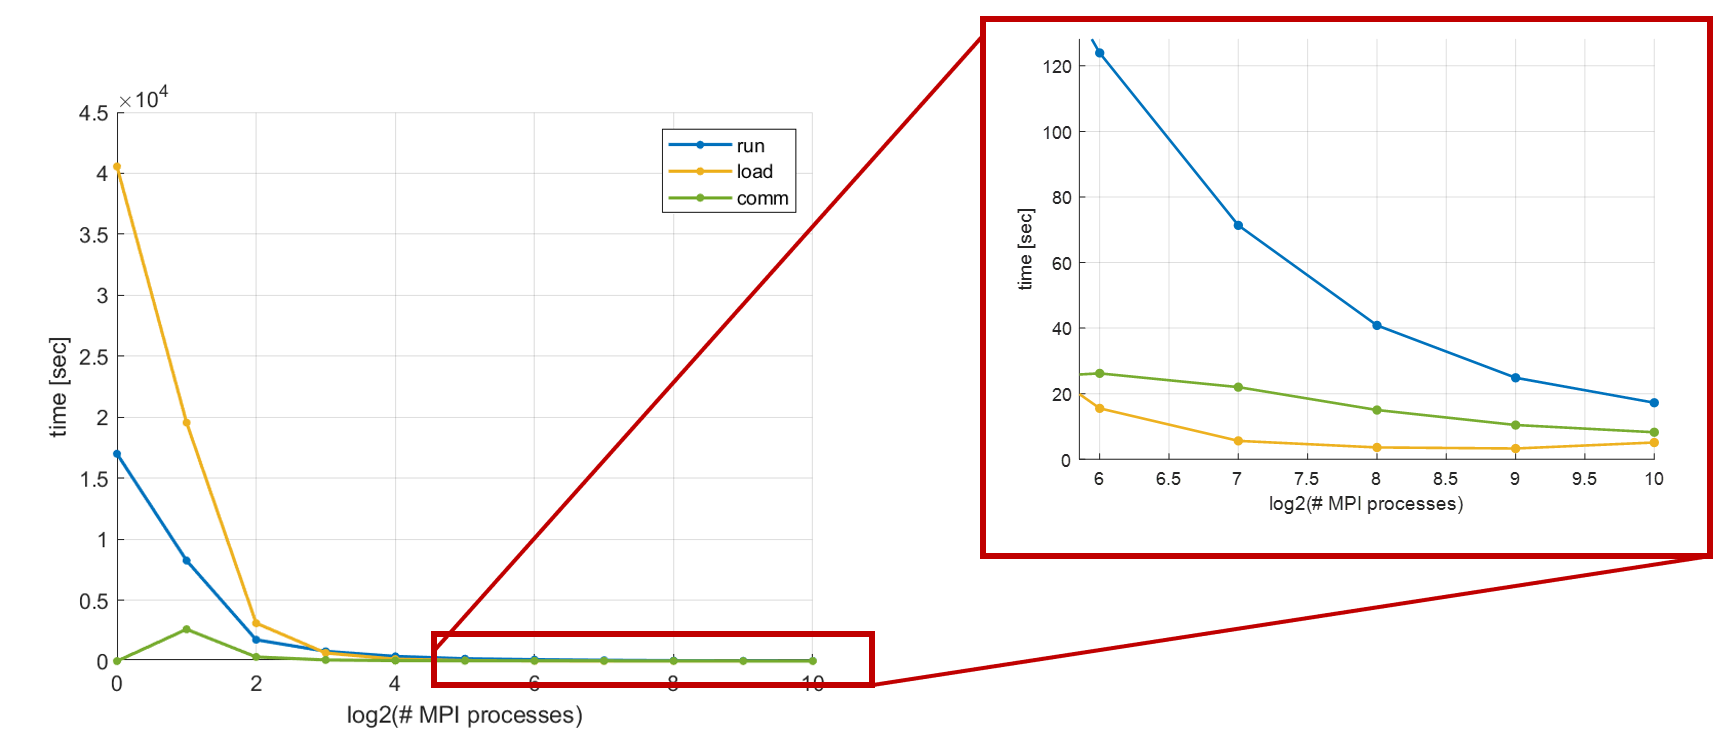
\includegraphics[width=\columnwidth]{figs/mpirun.png}
    \caption{CAPTION.}
    \label{fig:mpirun}
\end{figure}


\vspace{1in}


We ran OTM simulations on a Cray XC40 Cori supercomputer at NERSC~\cite{Cori}. Each node has two sockets, each socket is
populated with a 16-core Intel\textcopyright~Xeon\texttrademark~Processor E5-2698 v3 (``Haswell'') at 2.3 GHz and 128 GB of RAM memory. This is a very modern parallel computer, taking advantage of recent technology advances in parallel computers. 








% \subsection{Extra-Projection Method}
% The Extra-Projection method is an algorithm used to solve the dynamic user equilibrium problem. The inputs to the problem are a traffic network and a set of traffic demand $d_w : [0,T]\rightarrow \mathbb{R}^+ $, where $w\in\mathcal{W}$ is the set of origin destinations (OD) pairs. A solution $h$ is vector of demand on all available $ p\in\mathcal{P}$, where $h_p$ is the demand on path $p$. An optimal solution is a solution that creates a Wardrop traffic equilibrium \cite{wardrop1952some}. 

% EPM is based on the Euclidean projection defined as $\Pi_\mathcal{H}(x) = \underset{h}{\text{argmin}}\{\lvert h-x\rvert_2 \; : \;h \in\mathcal{H} \}$ and convergences when the travel cost function $F$ is Lipschitz continuous and pseudo-monotone. EMP has the following steps \cite{nie2010solving}:
% \begin{enumerate}
%     \item Start with an initial feasible solution $h^{1}$, set $k=1$ and set $\tau^1$ to a value less than the Lipschitz constant of $F$
%     \item Stop if $\frac {\langle c^k,y^k-h^k \rangle}{\langle y^k, c^k\rangle} \leq \epsilon$, where $c^k$ is a vector of travel cost $c_p^k$ for each path  $ p\in\mathcal{P}$ given demand $h^k$ and $y^k$ is the all-or-nothing assignment.
%     \item Determine $h^{k+1} = \Pi_\mathcal{H}(h^k - \tau^k F(z^k))$, and go back to step (2).
% \end{enumerate}

% The most time-consuming steps of the above algorithm are step 2 when calculating the all-or-nothing assignment, and steps 3 and 4 when performing the projection. This is because they involve looping over all the OD pairs, to determine the shortest path in step 2 and euclidean projection for step 3 and 4. Given $N$ computing cores, parallel computation is used to distribute the $\mathcal{W}$ od pairs among the $N$ cores such that each compute core performs step 2, 3 and 4 for $\mathcal{W}/N$ od pairs. 
